\documentclass{article}

\usepackage{graphicx}

\graphicspath{ {./images/} }

%All LaTeX documents have a ``preamble'' that includes the packages and macros needed to make the document compile. The file `PomonaLgcsFormatting.tex' includes the preamble for this template. You can see it in the file list on the left frame of your screen, and this document is instructed to use it with the \input{} command below.

\title{A Neighborhood classification and recommendation system}
\author{Gabriel Eduardo de Lima Machado}
\date{\today} 

\begin{document}

\maketitle

\begin{abstract}

This is the final project for the Coursera-IBM Data Science capstone. Its main propose is to train and use the skills learned along the course. In this project we will try to build a recommendation system that is able to find the most similar neighborhood in one city given another one in another city, using data from the venues in this cities.   

\end{abstract}

\section{Introduction}

\subsection{Background}
Recommendation systems are broadly used now days and they aim to spare us the time analyzing a lot of data and finding what is related to what. While this problem is always a matter of taste, because no system can ever predict exactly what someone wants to watch, or visit or buy, they can at least do a good job filtering the data and reducing the personal analysis. 

\subsection{The problem}
Imagine that person \emph{A} wants to visit a new city, given that this city is too big, this person does not have the time to look for all the places she could go and visit inside the city. More than that, she doesn't even know what exactly she wants to see there. However, person \emph{A} have been to a lot of places and she knows which ones she liked. With that in mind, can we based on some data build a model that is capable of predicting the places she would probably like to see?

\subsection{Interest}
There is plenty of persons \emph{A} around there the could make good use of such a system.

\section{Data acquisition}
\subsection{Data sources}
In this project we used the data provided by Foursquare by the means of their API based on URL queries. With this tool, we queried the data from the most recommended places in neighborhoods of Toronto and New York, this includes restaurants, bars, coffee shops, gyms, parks and related.

\subsection{Data use}
The data would be used to compare any neighborhood in Toronto with all the neighborhoods of Manhattan and choose the one that is more alike the first, or the one which the places are more similar.

\subsection{data cleaning}
We removed the places that where found only in one city but not in the other, while it can cause some distortion on the perception of the place, including these places could also lead to problems, so we decided to remove them,

\subsection{feature selection}
The only feature chosen from the venues was it's category, if it is a bar or a restaurant, etc.

\section{Exploring the data}
\subsection{Finding most commom places}
We counted the venues in both cities and found the most common venues categories and ploted them in the figure \ref{commom_man}. We also did the same for the Toronto ones that can be seen in the figure \ref{commom_tor}.

\begin{figure}[h!]
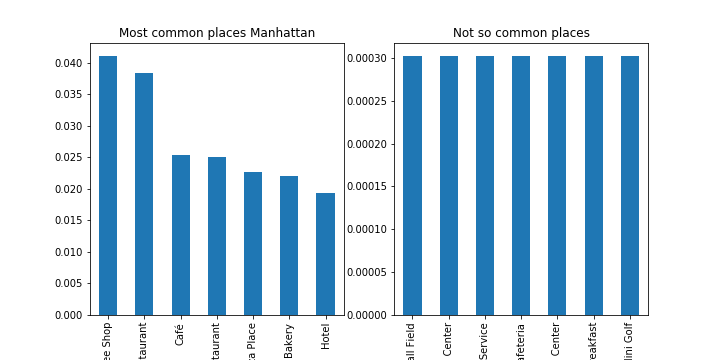
\includegraphics[width=10cm]{Common_manhattan.png}
\label{commom_man}
\caption{Manhattan Venues bar chart}
\end{figure}


\begin{figure}[h!]
	\includegraphics[width=10cm]{Common_toronto.png}
	\label{commom_tor}
	\caption{Toronto Venues bar chart}
\end{figure}

We can see that in both cases the coffee shops, restaurants and cafes are the most common venues. We can see that they also have some inter class correlation by the dotted graph in figure \ref{dotted}.

\begin{figure}[h!]
	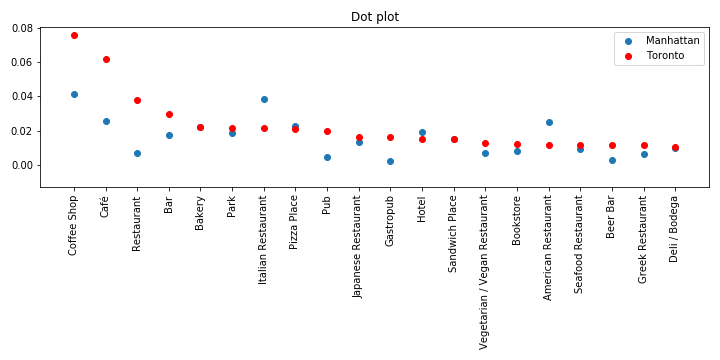
\includegraphics[width=10cm]{dotted_toronto.png}
	\label{dotted}
	\caption{Dotted chart}
\end{figure}

\subsection{data preparation}
The Venues the were not found in both cities were taken of from the dataframes and the categorical variables were transformed into dummie ones, them they were grouped by neighborhood and the mean  was taken from each category.

\section{Modeling}
\subsection{KNN algorithm}

The KNN algorithm is a supervised method of classification used to classify items that by distance. The samples are labeled with a class if it's the class that has the \emph{N} closest training samples. In this project we used the KNN model in the following manner:
\begin{itemize}
	\item The Manhattan samples are used to train the model. With the dummie categorical means being the training vectors.
	\item The labels for each vector is its neighborhood.
\end{itemize}

\subsection{Implementation}
Using the sklearn library we easily implemented the algorithm and each Toronto Neighborhood was assigned to a neighborhood in Manhattan. It is important to note that more than one neighborhood in Toronto can be assigned to the same one in Manhattan. Indeed, there was 40 different neighborhoods in Manhattan and only 19 of them were assigned as labels for the 73 neighborhoods in Toronto. This can be seen in the figure \ref{barh}.

\begin{figure}[h!]
	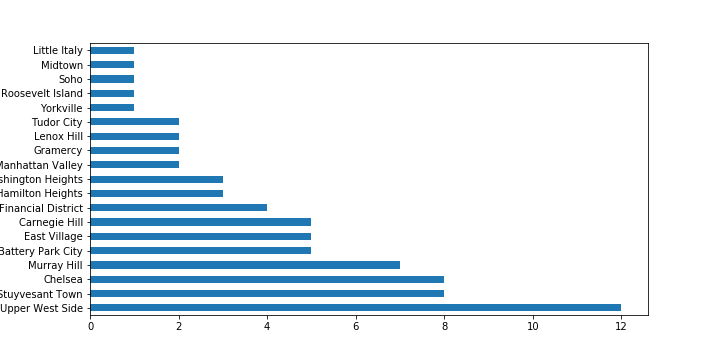
\includegraphics[width=10cm]{barh.png}
	\label{barh}
	\caption{Horizontal bar chart showing the distribution of the labels}
\end{figure}

\subsubsection{Results}
It's hard to compare the results as the similarity of places can be very subjective, but we can try to analyze some graphs and see that what was intended (label neighborhoods using euclidean distance) was indeed accomplished. Looking at the graphs in figure \ref{comp_plot} it's possible to analyze the places were the bars overlap each other. The labels were omitted for the sake of cleanliness. 

\begin{figure}[h!]
	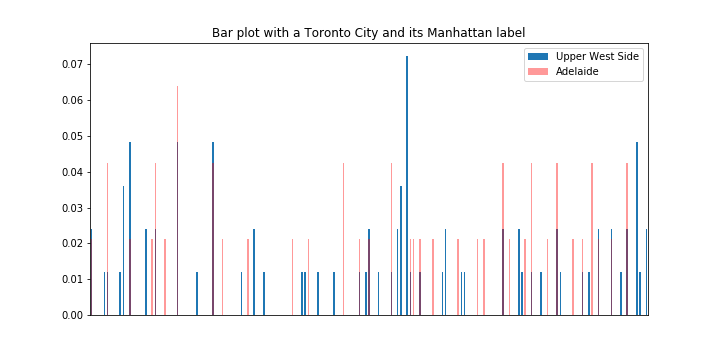
\includegraphics[width=10cm]{comparassion_plot.png}
	\label{comp_plot}
	\caption{Bar plot to show the similarity between the neighborhoods}
\end{figure}

\section{Discussion}
The project was based just in Venues categories, it would be important to include other characteristics such as  prices and rating. Another important thing is that a lot of venues have more than one category like 'Italian Restaurant' it is a restaurant and has Italian food, but in the current approach we are not considering that, we are  treating a 'Italian Restaurant' and a 'Restaurant' as completely different things, but it of course doesn't seems to be completely correct.   

\section{Conclusions}
The project is based in an heuristic assumption that the distance from means of venue's categories can lead to similarity between samples, which may not be true. One advantage of this approach is its easily implementation and the fact that we can change the weighs of each category if it's necessary. We can also easily do something like chose $N$ neighborhoods and finding another one the is more alike those three. Despite its simple model, the project can be a start point for a good recommendation system.

\end{document}